% Paquets généraux
\documentclass[a4paper,12pt,titlepage,twoside]{article}
\usepackage[T1]{fontenc}
\usepackage[utf8]{inputenc}
\usepackage[french]{babel}
\addto\captionsfrench{%
  \renewcommand{\tablename}{Tableau}%
}
\usepackage[gen]{eurosym}
%\usepackage[dvips]{graphicx}
\usepackage{fancyhdr}
\usepackage{pdfpages} 
\usepackage{multido}
\usepackage{hyperref}
%\usepackage{textcomp}
\usepackage{schemabloc}
\usepackage[bitstream-charter]{mathdesign}
\usepackage{array}
\newcolumntype{P}[1]{>{\centering\arraybackslash}p{#1}}

\newcommand{\id}{54}
\newcommand{\nom}{Liaisons mécaniques}
\newcommand{\sequence}{04}
\newcommand{\num}{01}
\newcommand{\type}{TP}
\newcommand{\descrip}{Modélisation d'un solide. Comportement des liaisons mécaniques. Modéliser les mécanismes du laboratoire par un schéma cinématique, paramétré.}
\newcommand{\competences}{A3-C4: Analyse d'architecture et de comportement \\ &  Mod1-C1: Isolement d'un solide ou d'un système de solides \\ &  Mod2-C10-1: Modèle de solide indéformable \\ &  Mod2-C11: Modélisation géométrique et cinématique des mouvements entre solides indéformables \\ &  Mod2-C12: Modélisation cinématique des liaisons entre solides \\ &  Mod2-C15: Modélisation des actions mécaniques \\ &  Rés-C6: Utilisation d'un solveur ou d'un logiciel multi physique \\ &  Com1-C1: Différents descripteurs introduits dans le programme \\ &  Com2-C4: Outils de communication}
\newcommand{\nbcomp}{9}
\newcommand{\systemes}{Plateforme Stewart}
\newcommand{\systemessansaccent}{Plateforme Stewart}
\newcommand{\ilot}{2}
\newcommand{\ilotstr}{02}
\newcommand{\dossierilot}{\detokenize{Ilot_02 Plateforme Stewart}}
\newcommand{\imageun}{Plateforme}

\newcommand{\urlsysteme}{\href{https://www.costadoat.fr/systeme/57}{Ressources système}}
\newcommand{\matlabsimscape}{\href{https://github.com/Costadoat/Sciences-Ingenieur/raw/master/Systemes/Plateforme Stewart/Plateforme_Stewart_Simscape.zip}{Modèle Simscape}}
\newcommand{\solidworks}{\href{https://github.com/Costadoat/Sciences-Ingenieur/raw/master/Systemes/Plateforme Stewart/Plateforme_Stewart_Solidworks.zip}{Modèle Solidworks}}
\newcommand{\edrawings}{\href{https://github.com/Costadoat/Sciences-Ingenieur/raw/master/Systemes/Plateforme Stewart/Plateforme_Stewart.EASM}{Modèle eDrawings}}
\newcommand{\test}{Stewart_param1}
\newcommand{\testi}{Stewart_param2}
\newcommand{\testii}{Stewart_param3}
\newcommand{\testiii}{Stewart_param4}
\newcommand{\testiiii}{Stewart_euler}

\newcommand{\institute}{Lycée Dorian}

\usepackage{fancyvrb}
\usepackage{color}
\usepackage{xcolor}
\usepackage{colortbl}
\usepackage{helvet}
\renewcommand{\familydefault}{\sfdefault}
\usepackage{amsfonts}
\usepackage{amsmath}
%\usepackage{xspace}
\usepackage{varioref}
\usepackage{tabularx}
%\usepackage{floatflt}
\usepackage{graphics}
\usepackage{wrapfig}
\usepackage{textcomp}
\usepackage{tikz}
\usepackage{wrapfig}
\usepackage{gensymb}
\usepackage[percent]{overpic}
\usepackage[european]{circuitikz}
\usetikzlibrary{babel}
\usepackage{ifthen}
\usepackage{cancel}
\usepackage{etoolbox}
\usepackage{multirow}
%\usepackage{boxedminipage}
\definecolor{gris25}{gray}{0.75}
\definecolor{bleu}{RGB}{18,33,98}
\definecolor{bleuf}{RGB}{42,94,171}
\definecolor{bleuc}{RGB}{231,239,247}
\definecolor{rougef}{RGB}{185,18,27}
\definecolor{rougec}{RGB}{255,188,204}%255,230,231
\definecolor{vertf}{RGB}{103,126,82}
\definecolor{vertc}{RGB}{220,255,191}
\definecolor{forestgreen}{rgb}{0.13,0.54,0.13}
\definecolor{blcr}{rgb}{0.59,0.69,0.84}
\definecolor{blfr}{rgb}{0.32,0.51,0.75}
\definecolor{orfr}{rgb}{0.90,0.42,0.15}
\definecolor{orcr}{rgb}{0.90,0.65,0.50}
\definecolor{orangef}{rgb}{0.659,0.269,0.072}
\definecolor{orange}{rgb}{0.58,0.35,0.063}
\definecolor{orangec}{rgb}{0.43,0.32,0.25}
\definecolor{rcorrect}{rgb}{0.6,0,0}
\definecolor{sequence}{rgb}{0.75,0.75,0.75}
\definecolor{competences}{rgb}{0.61,0.73,0.35}
\definecolor{grisf}{HTML}{222222}
\definecolor{grisc}{HTML}{636363}
\definecolor{normal}{HTML}{4087c4}
\definecolor{info}{HTML}{5bc0de}
\definecolor{success}{RGB}{92,184,92}
\definecolor{warning}{RGB}{240,173,78}
\definecolor{danger}{RGB}{217,83,79}
\hypersetup{                    % parametrage des hyperliens
    colorlinks=true,                % colorise les liens
    breaklinks=true,                % permet les retours à la ligne pour les liens trop longs
    urlcolor= blfr,                 % couleur des hyperliens
    linkcolor= orange,                % couleur des liens internes aux documents (index, figures, tableaux, equations,...)
    citecolor= forestgreen                % couleur des liens vers les references bibliographiques
    }

% Mise en page
\pagestyle{fancy}

\setlength{\hoffset}{-18pt}
\setlength{\oddsidemargin}{0pt} 	% Marge gauche sur pages impaire2s
\setlength{\evensidemargin}{0pt} 	% Marge gauche sur pages paires
\setlength{\marginparwidth}{00pt} 	% Largeur de note dans la marge
\setlength{\headwidth}{481pt} 	 	% Largeur de la zone de tête (17cm)
\setlength{\textwidth}{481pt} 	 	% Largeu\textbf{r de la zone de texte (17cm)
\setlength{\voffset}{-18pt} 		% Bon pour DOS
\setlength{\marginparsep}{7pt}	 	% Séparation de la marge
\setlength{\topmargin}{-30pt} 		% Pas de marge en haut
\setlength{\headheight}{55pt} 		% Haut de page
\setlength{\headsep}{20pt} 		% Entre le haut de page et le texte
\setlength{\footskip}{30pt} 		% Bas de\textbf{ page + séparation
\setlength{\textheight}{700pt} 		% Hauteur de l'icone zone de texte (25cm)
\setlength\fboxrule{1 pt}
\renewcommand{\baselinestretch}{1}
\setcounter{tocdepth}{1}
\newcommand{\cadre}[2]
{\fbox{
  \begin{minipage}{#1\linewidth}
   \begin{center}
    #2\\
   \end{center}
  \end{minipage}
 }
}

\newcommand{\repon}[1]
{
~\ \\
\begin{tabular}{|m{\linewidth}|}
 \hline
\multido{}{#1}{\\ \hline}
\end{tabular}
}

\newcounter{num_quest} \setcounter{num_quest}{0}
\newcounter{num_rep} \setcounter{num_rep}{0}
\newcounter{num_cor} \setcounter{num_cor}{0}

\newcommand{\question}[1]{\refstepcounter{num_quest}\par
~\ \\ \parbox[t][][t]{0.15\linewidth}{\textbf{Question \arabic{num_quest}}}\parbox[t][][t]{0.85\linewidth}{#1}\par
}


\newcommand{\reponse}[3]
{\refstepcounter{num_rep}
\noindent
\rule{\linewidth}{.5pt}\\
\textbf{Question \arabic{num_rep}:} ~\ \\
\ifdef{\public}{\multido{\i=1+1}{#1}{~\ \\}#2}{#3}
}

\newcommand{\cor}
{\refstepcounter{num_cor}
\noindent
\rule{\linewidth}{.5pt}
\textbf{Question \arabic{num_cor}:} \\
}

\newcommand{\repcarre}[2]
{
~\ \\
\begin{tikzpicture}
\draw [fill=white] (0,0) rectangle +(\linewidth,#1);
\node[align=left] at (1.1,#2-0.3) {\textbf{Question #1:}};
\end{tikzpicture}
}

\newcommand{\titre}[1]
{\begin{center}
\cadre{0.8}{\huge #1} 
\end{center}
}


% En tête et pied de page
\lhead{\nom}
\rhead{
\includegraphics[width=2cm]{../../img/logo}}
\lfoot{\auteurun,\ \auteurdeux}
\cfoot{Page \thepage}

\fancypagestyle{documentreponse}{%
  \fancyhf{}
  \fancyhead[LO]{Nom: ........................ Prénom: ........................}
  \fancyhead[LE]{\nom}
  \fancyhead[RE,RO]{
\includegraphics[width=2cm]{../../img/logo}}
  \lfoot{Document réponse}
  \cfoot{Page \thepage}
   }
  
\fancypagestyle{correction}{%
  \fancyhf{}
  \lhead{\colorbox{danger}{\begin{minipage}{0.65\paperwidth} \textcolor{white}{\textbf{Correction}} \end{minipage}} }
  \rhead{
\includegraphics[width=2cm]{../../img/logo}}
  \lfoot{Renaud Costadoat, Françoise Puig}
  \rfoot{\colorbox{danger}{\begin{minipage}{0.5\paperwidth} \begin{flushright}\textcolor{white}{\textbf{Correction}}\end{flushright} \end{minipage}} }}

\fancypagestyle{correctioninfo}{%
  \fancyhf{}
  \lhead{\colorbox{danger}{\begin{minipage}{0.65\paperwidth} \textcolor{white}{\textbf{Correction}} \end{minipage}} }
  \rhead{
\includegraphics[width=2cm]{../../img/logo}}
  \lfoot{Renaud Costadoat, Juliette Genzmer, Willie Robert}
  \rfoot{\colorbox{danger}{\begin{minipage}{0.6\paperwidth} \begin{flushright}\textcolor{white}{\textbf{Correction}}\end{flushright} \end{minipage}} }}

\renewcommand{\footrulewidth}{0.4pt}

\usepackage{eso-pic}
\newcommand{\BackgroundPic}{%
\put(0,0){%
\parbox[b][\paperheight]{\paperwidth}{%
\vfill
\begin{center}
\hspace{0.5cm}\vspace{0.5cm}

\includegraphics[width=\paperwidth,height=\paperheight,%
keepaspectratio]{../../img/fond3}%
\end{center}
\vfill
}}}

\newcommand{\BackgroundPicdeux}{%
\put(25,-30){%
\parbox[b][\paperheight]{\paperwidth}{%
\vfill
\begin{center}

\includegraphics[width=\paperwidth,height=\paperheight,%
keepaspectratio]{../../img/fond4}%
\end{center}
\vfill
}}}

\begin{document}

\pagestyle{empty}

\AddToShipoutPicture*{\BackgroundPic}


\includegraphics[width=2cm]{../../img/logo}

\Huge{DS \num\ - \sujet}

\vspace{1cm}

\ifdef{\prive}{\begin{center}\colorbox{danger}{\Huge{Avec Correction}}\end{center}}{}

\begin{center}
\centering\huge{PTSI}
\end{center}

\vspace{2cm}


\begin{center}
\centering\Large{\jour}
\end{center}

\vspace{2cm}

\normalsize

\tableofcontents

\newpage

\AddToShipoutPicture{\BackgroundPicdeux}

\pagestyle{fancy}

\begin{center}
\Huge \sujet
\end{center}


\normalsize

\section{Présentation}

Chaque année, 65 millions de parfums, 57 millions d’unités de soins et 37 millions d’unités de maquillage sont produits sur le site Parfums Christian Dior à Saint-Jean-de-Braye, à proximité d’Orléans. Environ 1 700 personnes travaillent sur le site. Celui-ci, d’une superficie de 55 hectares, accueille les services de production, de ventes, d’expédition, administratifs ainsi que le centre de recherche LVMH. Les recettes qui ont fait, et qui font actuellement, le succès de la maison Christian Dior sont très caractéristiques du milieu du luxe : créativité, qualité, passion, innovation, culture, notion du rêve et sensibilité artistique. L’automatisation des systèmes de production s’avère un atout indispensable ; la recherche de la qualité optimale et l’augmentation constante de la production nécessitent de supprimer les tâches manuelles pénibles, ou à risque de non qualité.

\paragraph{Création de motifs sur du blush}

Le blush est un produit cosmétique qui se présente sous forme de poudre compactée et qui s’applique sur le visage à l'aide d'un gros pinceau. La création de motifs sur le blush permet de rendre l'intérieur du boîtier de maquillage plus attrayant et immédiatement différentiable de celui des autres marques (figure \ref{img01}).

\begin{figure}[!h]
\centering
\includegraphics[width=0.65\linewidth]{img/fig01}
 \caption{Poudre de maquillage compactée avant et après création des motifs}
 \label{img01}
\end{figure}

\paragraph{Contexte de l’étude}

Le système étudié permet de créer des motifs par pulvérisations de solutions constituées de nacres et d’alcool sur des godets de poudre compactée.

\begin{figure}[!h]
\centering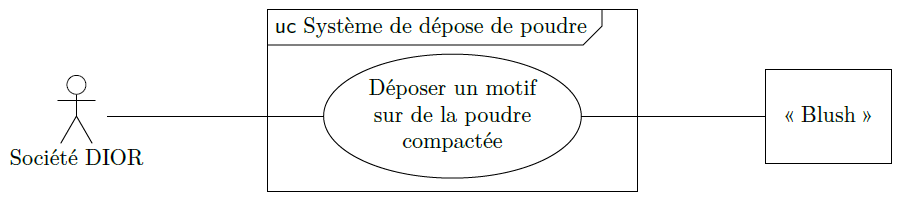
\includegraphics[width=0.8\linewidth]{img/fig02}
 \caption{Diagramme des cas d’utilisation du système}
 \label{img02}
\end{figure}

La création de motifs se fait en deux étapes :
\begin{itemize}
 \item la première étape consiste, en utilisant un masque (pochoir), à pulvériser la solution nacrée à l’aide de buses de pulvérisation (spray) à jets larges,
 \item la deuxième étape permet de créer les motifs fins par pulvérisation à l’aide de buses de pulvérisation à aiguille.
\end{itemize}

Le système de pulvérisation de nacres (figure \ref{img06}) comporte :
\begin{itemize}
 \item un plateau tournant sur huit postes pour la pulvérisation large et fine (figure \ref{img07}),
 \item un poste de lavage et séchage des masques après pulvérisation à jets larges,
 \item deux bras munis de pinces qui permettent le transfert des masques propres et usagés entre le plateau tournant et le poste de lavage.
\end{itemize}

\begin{figure}[!h]
\centering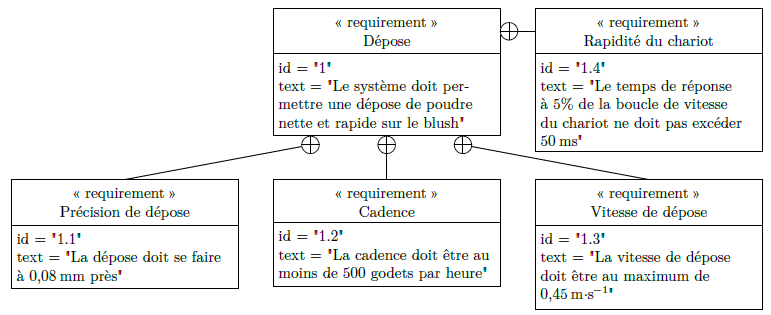
\includegraphics[width=0.8\linewidth]{img/fig03}
 \caption{Diagramme des exigences du système}
 \label{img03}
\end{figure}

\begin{figure}[!h]
\centering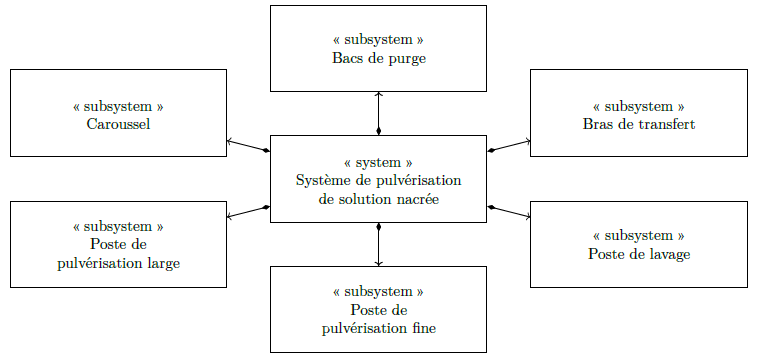
\includegraphics[width=0.8\linewidth]{img/fig04}
 \caption{Diagramme de définition des blocs du système de pulvérisation de solution nacrée}
 \label{img04}
\end{figure}

Avant chaque début de cycle, les buses sont automatiquement purgées dans les bacs prévus à cet effet.

Pour un plateau contenant les godets de poudre compactée, la création de motifs se déroule suivant le cycle ci-dessous :
\begin{itemize}
 \item convoyage et indexage du plateau contenant les godets de poudres compactées sur le poste de chargement,
 \item rotation puis dépose du masque propre sur le plateau à godets,
 \item rotation puis pulvérisation large,
 \item rotation puis prise du masque sale,
 \item trois rotations puis pulvérisation fine,
 \item rotation et déchargement du plateau à godets.
\end{itemize}

Lors des pulvérisations, les buses sont fixes, le support sur lequel est indexé le plateau à godets est mobile et asservi en position suivant deux axes (pulvérisation large) ou trois axes (pulvérisation fine).

Le poste de pulvérisation fine est constitué d’un robot cartésien suivant 3 directions de l’espace. Ce sujet a pour objectif de vérifier que la construction du poste de pulvérisation permet d’atteindre les exigences présentées sur le diagramme de la figure \ref{img03}, plus particulièrement suivant un axe que l’on appellera l’axe $\overrightarrow{x}$ (figure \ref{img08}).

\begin{figure}[!h]
\centering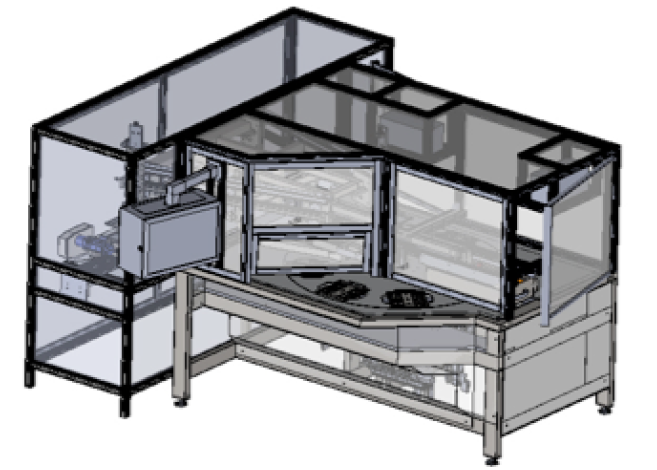
\includegraphics[width=0.7\linewidth]{img/fig05}
 \caption{Vue de l’installation}
 \label{img05}
\end{figure}

\begin{figure}[!h]
\centering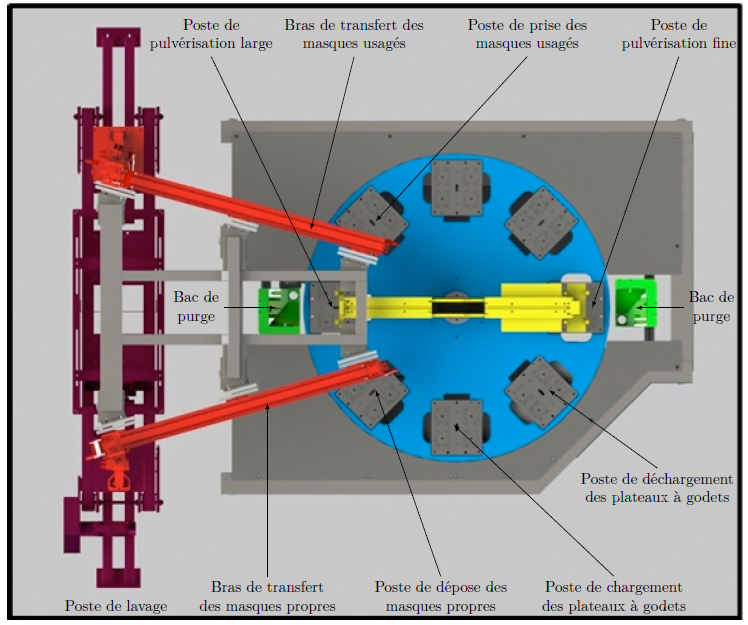
\includegraphics[width=0.7\linewidth]{img/fig06}
 \caption{Système de pulvérisation des nacres}
 \label{img06}
\end{figure}

\begin{figure}[!h]
\centering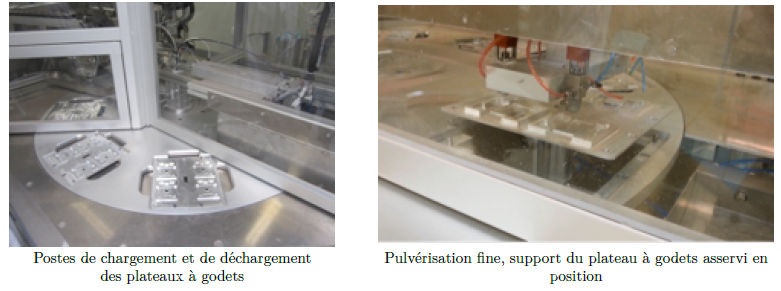
\includegraphics[width=0.95\linewidth]{img/fig07}
 \caption{Photos de postes}
 \label{img07}
\end{figure}

\section{Modélisation de la chaine cinématique du déplacement du préhenseur suivant l’axe x}

\paragraph{Objectif}

L’objectif de cette partie est de proposer un modèle du mécanisme constituant le déplacement de l’axe $\overrightarrow{x}$ et de justifier certains choix technologiques.

Le préhenseur repose sur des plaques support (figure \ref{img08}) qui le lient en liaison encastrement au bâti. Les rails guidant le préhenseur suivant l’axe $\overrightarrow{x}$ supportent les autres rails guidant les déplacement du préhenseur suivant les axes $\overrightarrow{y}$ et $\overrightarrow{z}$.

\begin{figure}[!h]
\centering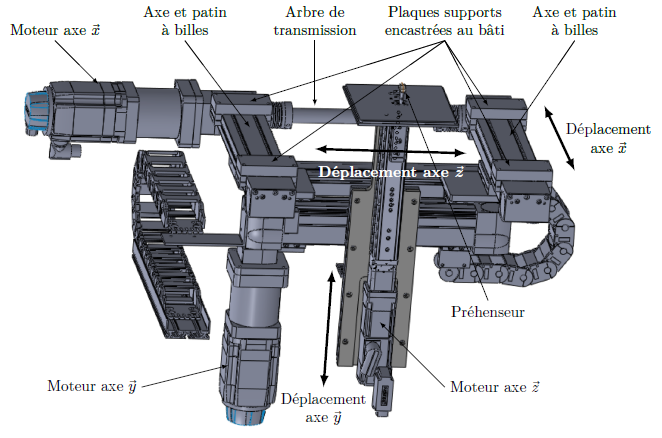
\includegraphics[width=0.75\linewidth]{img/fig08}
 \caption{Architecture des différents axes}
 \label{img08}
\end{figure}

Le guidage est réalisé par deux axes munis de patins à billes (figures \ref{img09}). Le moteur actionnant l’axe x est lié à un réducteur qui entraîne deux ensembles poulies-courroies. Les poulies motrices sont guidées chacune par deux roulements à billes. Les deux poulies motrices sont liées par un arbre de transmission (Arbre 1).

\begin{figure}[!h]
\centering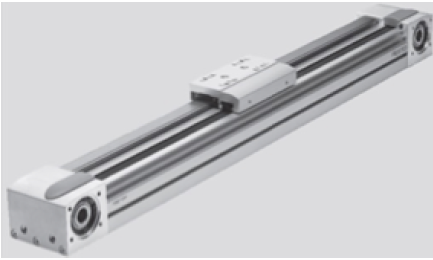
\includegraphics[width=0.7\linewidth]{img/fig09}
 \caption{Axe et patin à billes}
 \label{img09}
\end{figure}

\newpage

Données:
\begin{itemize}
 \item $\Phi=28,65mm$ est le diamètre primitif des poulies,
 \item $r=\frac{\omega_{poulie}}{\omega_{moteur}}=\frac{\theta_{poulie}}{\theta_{moteur}}=\frac{1}{10}$ : rapport de réduction du réducteur entre le moteur et les poulies.
\end{itemize}

Un capteur angulaire permet de mesurer la position angulaire du moteur $cap_{moteur}$.

\question{Colorier les classes d'équivalence du système sur le document réponse. (ne pas colorier la courroie qui ne peut être considérée comme une classe d'équivalence car flexible).}

\question{Déterminer la précision angulaire notée $\delta\theta_{moteur}$ nécessaire au niveau du capteur $cap_{moteur}$, qui permettrait de valider l'exigence \verb?id='1.1'?.}

\section{Validation de la sensibilité du capteur de position de l’axe x et de son circuit de mise en forme}

\paragraph{Objectif}

L’objectif de cette partie est, au vu du cahier des charges, de valider les choix proposés et les réglages des constituants qui permettent d’acquérir l’information de position.

Afin de permettre le pilotage par le variateur de vitesse, la résolution sur la mesure de la position angulaire du rotor de la machine synchrone doit être de 15 minutes d’angle soit $\Delta\theta_{max} = (15/60)\textdegree$. De plus, via un traitement
incrémental, la résolution sur la mesure de déplacement du plateau à godets suivant l’axe $\overrightarrow{x}$ doit être meilleure que $\Delta x_{max} = 37 \mu m$. Le rapport de transmission est $K_1 = 1,4325\cdot 10^{-3} m\cdot rad^{-1}$.

La structure utilise un résolveur bipolaire accouplé directement sur l’arbre de la machine électrique. Le résolveur bipolaire est un transformateur, sans bague, ni balais, qui se compose essentiellement d’un enroulement primaire et de deux enroulements secondaires orthogonaux aux bornes desquels on trouve les tensions $v_1$ et $v_2$ (figure 13). Le rapport de transformation entre l’enroulement primaire et les deux enroulements secondaires est noté $m = \frac{1}{2}$.

$\frac{d\theta}{dt}=\Omega$ est la vitesse de rotation angulaire du rotor de la machine électrique, l’étude se fait à vitesse $\Omega$ constante, $\theta(0) = 0$.

Une tension d’excitation sinusoïdale, $v_r(t)=V_{r\  max}\cdot sin(2\cdot \pi\cdot f_r\cdot t)$, de fréquence $f_r=10kHz$, est appliquée à
l’enroulement primaire du résolveur (figure \ref{img11}).

\begin{figure}[!h]
\begin{minipage}{0.5\linewidth}
\centering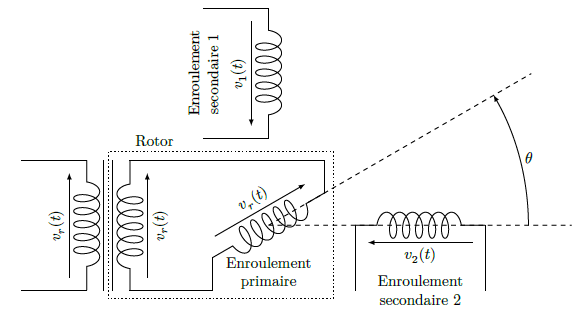
\includegraphics[width=0.9\linewidth]{img/fig10}
 \caption{Schéma de principe du résolveur}
 \label{img10}
\end{minipage}\hfill
\begin{minipage}{0.4\linewidth}
\centering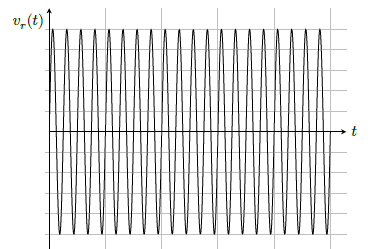
\includegraphics[width=0.9\linewidth]{img/fig11}
 \caption{Tension d’excitation}
 \label{img11}
\end{minipage}
\end{figure}

Les tensions $v_i(t)=m\cdot V_{r\ max}\cdot sin(2\cdot \pi\cdot f_r\cdot t)\cdot cos(\theta(t))$ et $v_j(t)=m\cdot V_{r\ max}\cdot sin(2\cdot \pi\cdot f_r\cdot t)\cdot sin(\theta(t))$ induites dans les enroulements fixes des deux secondaires sont modulées en fonction des variations de l’angle mécanique $\theta$ (figure \ref{img12}).

\begin{figure}[!h]
\centering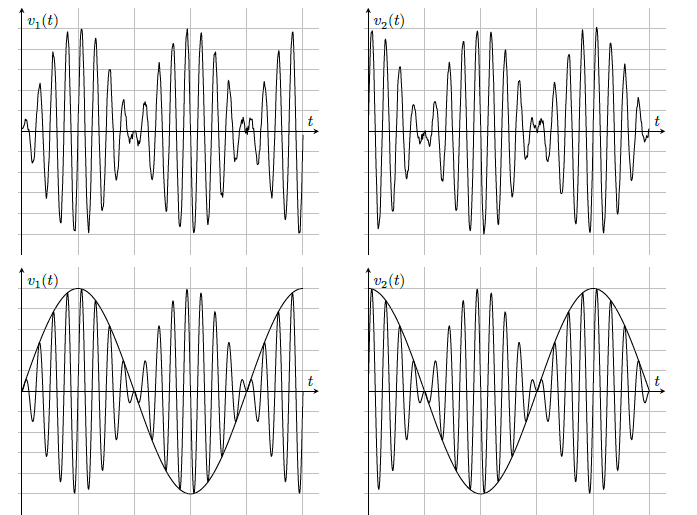
\includegraphics[width=0.7\linewidth]{img/fig12}
 \caption{Tensions $v_1(t)$ et $v_2(t)$ bruitées (en haut) et filtrées (en bas) pour une vitesse de rotation $\Omega$ constante}
 \label{img12}
\end{figure}

\question{Identifier sur la figure \ref{img12} si [i,j]=[1,2] ou [i,j]=[2,1].}

\question{On écrit $\theta(t)=2\cdot\pi\cdot k_f\cdot f_r \cdot t$. Déterminer la valeur numérique de $k_f$ graphiquement.}

\section{Validation du choix de la motorisation permettant le déplacement selon l’axe x}

\paragraph{Objectif}

L’objectif est de valider le choix du moteur effectué par le concepteur du système.

Le cahier des charges impose que la vitesse maximale du chariot sur l’axe $\overrightarrow{x}$ soit de $V_{max}=0,45 m\cdot s^{-1}$ et que l’accélération maximale du chariot soit de $\gamma_{max}=10m\cdot s^{-2}$.

Notations
\begin{itemize}
 \item $\omega_m$ : vitesse de rotation du moteur,
 \item $u_m$ : tension d'alimentation du moteur,
 \item $i_m(t)$ courant électrique traversant le moteur,
 \item $r=\frac{n_{axe\ poulie}}{n_{moteur}}=\frac{1}{10}$ : rapport de réduction du réducteur entre le moteur et les poulies,
 \item $M_2=25kg$ : masse de l’ensemble mobile 2,
 \item $\Phi=28,65mm$ est le diamètre primitif des poulies,
 \item l’inertie des courroies est négligée,
 \item $J_m=1,2\cdot 10^{-5}kg\cdot m^2$ : moment d’inertie de l’arbre moteur,
 \item $J_1=4\cdot 10^{-4} kg\cdot m^2$ : moment d’inertie de l’arbre 1,
 \item $C_r$ : couple de frottements secs dans les liaisons ramené à l’arbre moteur,
 \item $\mu=0,001 N\cdot m\cdot s\cdot rad^{-1}$ : coefficient de frottements visqueux dans les liaisons ramené à l’arbre moteur,
 \item $Rm=2\Omega$ : résistance électrique interne du moteur,
 \item $Lm$: inductance du moteur négligée,
 \item $K_e=50\cdot 10^{-3}V\cdot rad^{-1}\cdot s$ : constance électrique du moteur,
 \item $K_c=50\cdot 10^{-3}N.\cdot m\cdot A^{-1}$ : constance de couple du moteur,
\end{itemize}

\question{Déterminer la vitesse maximale de rotation du moteur $\Omega_{max}$. Faire l’application numérique. (on pourra utiliser les figures \ref{img09} ainsi que le dessin du document réponse.}

\question{Déterminer l’accélération maximale du moteur $\dot{\Omega}_{max}$. Faire l’application numérique.}

On donne l'inertie équivalente ramenée à l'arbre moteur:

\begin{center}
$J=J_m+J_1\cdot r^2+\frac{M_2\cdot r^2\cdot \Phi^2}{4}$
\end{center}

\question{Faire l'application numérique à $10^{-1}$ près.}

On prendra pour la suite $J=6\cdot 10^{-5}kg.m^2$.

Le théorème du moment dynamique permet d'écrire:

\begin{center}
$J\cdot \frac{d\omega_m(t)}{dt}=c_m(t)-\mu\cdot \omega_m(t)-Cr$
\end{center}

\question{Montrer que cette équation est homogène.}

\question{Écrire les 3 équations temporelles du moteur qui s'ajoutent à la précédente.}

\question{Écrire ces 4 équations dans le domaine de Laplace.}

Pour la suite, on prendra $Cr=0$.

\question{Écrire la fonction de transfert 
$H(p)=\frac{\Omega_m(p)}{U_m(p)}$ sous la forme canonique.}

\question{Identifier l'ordre et la classe de la fonction de transfert.}

\question{Identifier les éléments caractéristiques de la fonction de transfert.}

\question{Faire l'application numérique.}

\question{Pour faire tourner le moteur à sa vitesse maximale, quelle doit être la tension $U_{max}$ en entrée ?}

Pour la suite, on prendra $U_0=25V$.

\question{Déterminer alors l'expression de $\omega_m(t)$, la réponse temporelle de $H(p)$ à un échelon d'amplitude $U_0$.}

\begin{figure}[ht!]
\begin{minipage}{0.47\linewidth}
\centering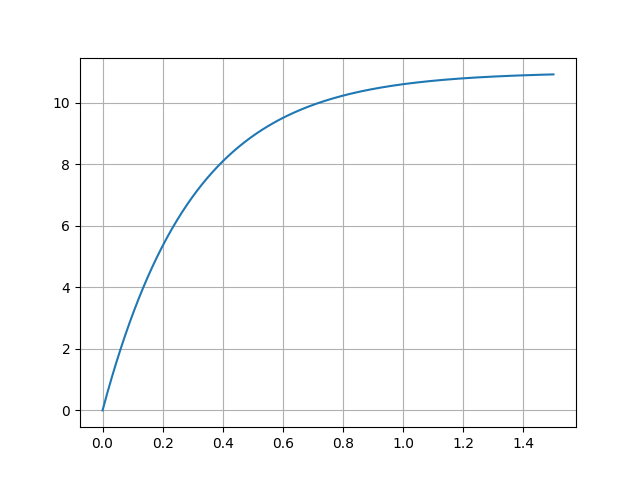
\includegraphics[width=0.95\linewidth]{img/fig13a}
 \caption{Tracé A}
 \label{img13a}
\end{minipage}\hfill
\begin{minipage}{0.47\linewidth}
\centering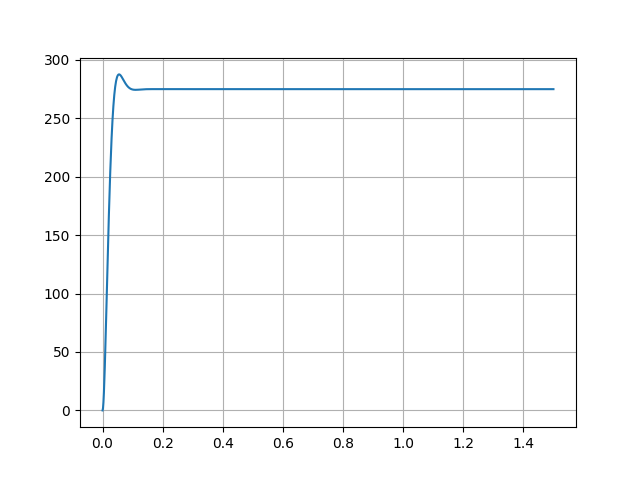
\includegraphics[width=0.95\linewidth]{img/fig13b}
 \caption{Tracé B}
 \label{img13b}
\end{minipage}\\
\begin{minipage}{0.47\linewidth}
\centering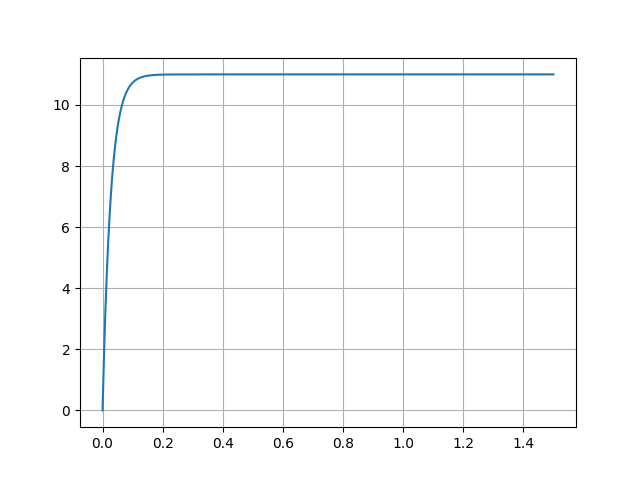
\includegraphics[width=0.95\linewidth]{img/fig13c}
 \caption{Tracé C}
 \label{img13c}
\end{minipage}\hfill
\begin{minipage}{0.47\linewidth}
\centering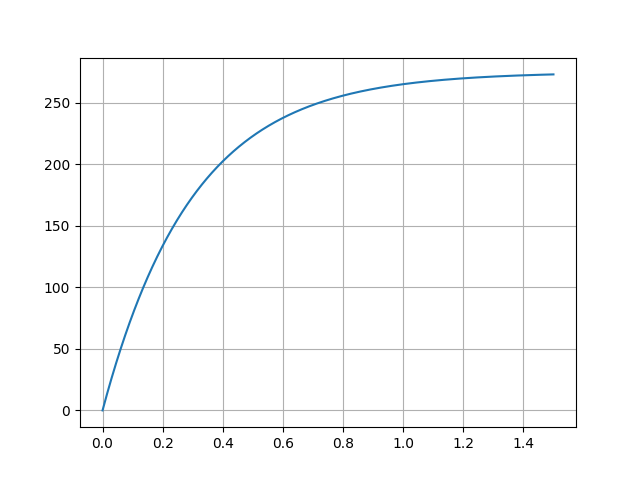
\includegraphics[width=0.95\linewidth]{img/fig13d}
 \caption{Tracé D}
 \label{img13d}
\end{minipage}\\
\begin{minipage}{0.47\linewidth}
\centering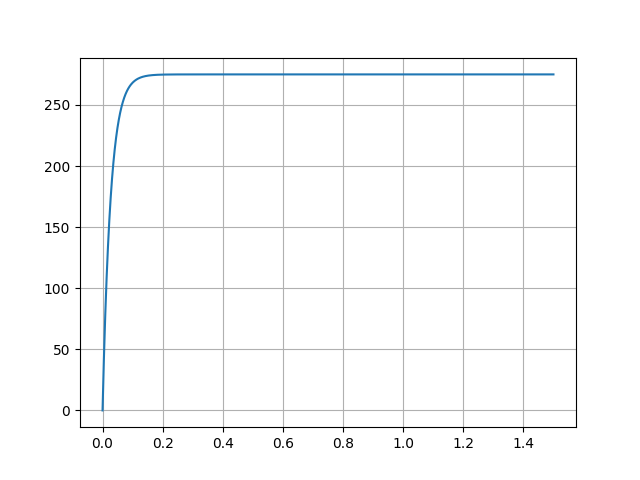
\includegraphics[width=0.95\linewidth]{img/fig13e}
 \caption{Tracé E}
 \label{img13e}
\end{minipage}\hfill
\begin{minipage}{0.47\linewidth}
\centering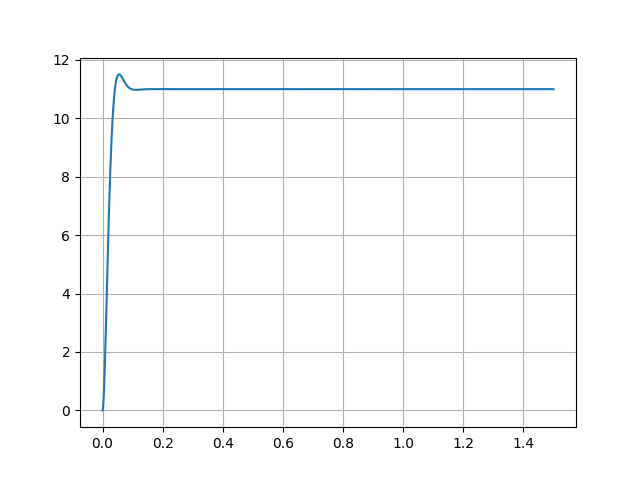
\includegraphics[width=0.95\linewidth]{img/fig13f}
 \caption{Tracé F}
 \label{img13f}
\end{minipage}
\end{figure}


\question{Les figures \ref{img13a} à \ref{img13f} présentent des réponses temporelles. Déterminer à laquelle correspond celle calculée précédemment. Justifier la réponse en indiquant pour chacune d'elle ce qui la différencie du résultat attendu}

\section{Identification d'une réponse temporelle}

On donne la réponse suivante $s(t)$ ($rad.s^{-1}$) pour un échelon $e(t)=6V$.

\begin{figure}[!ht]
\centering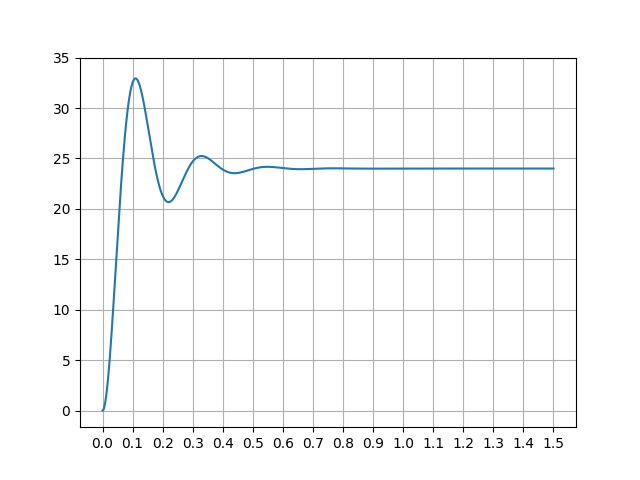
\includegraphics[width=0.8\linewidth]{img/fig14}
\caption{Tracé de la réponse temporelle s(t)}
\label{fig01}
\end{figure}

\question{Déterminer (le gain statique) $K$ de la fonction de transfert correspondante, vous préciserez l'unité.}

\question{Déterminer $\xi$ (à 0,1 près) de la fonction de transfert correspondante, vous préciserez l'unité. On donne $\left(\frac{ln(\frac{8}{3})}{\pi}\right)^2=0,1$.}

\question{Déterminer $\omega_0$ de la fonction de transfert correspondante, vous préciserez l'unité.}

\cleardoublepage

\ifdef{\public}{\pagestyle{documentreponse}}{\pagestyle{correction}}


\reponse{0}{\begin{center}
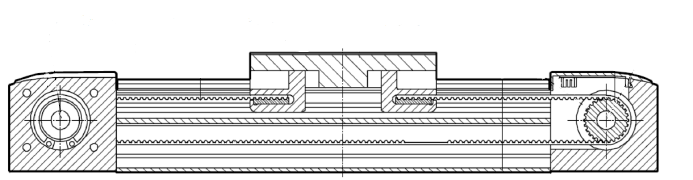
\includegraphics[width=0.9\linewidth]{img/DR_q1}
\end{center}}{
\begin{center}
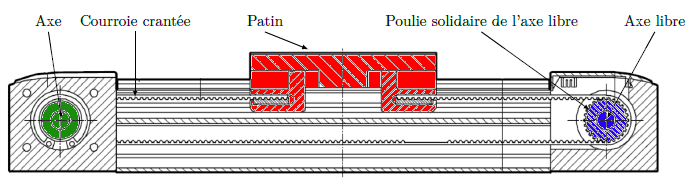
\includegraphics[width=0.9\linewidth]{img/DR_q1_cor}
\end{center}}

\reponse{6}{}{
$\delta x=0.08mm=\frac{\Phi}{2}\cdot \delta\theta_{poulie}
=\frac{\Phi}{2}\cdot r \cdot \delta\theta_{moteur}$

Donc, $\delta\theta_{moteur}=\frac{\delta x}{\frac{\Phi}{2}\cdot r}=\frac{0.08}{\frac{28.65}{2}\cdot \frac{1}{10}}=\frac{20\cdot 0.08}{28.65}\approx \frac{1.6}{28}\approx \frac{0.4}{7}\approx 0.055rad$.}

\reponse{2}{}{
[i,j]=[2,1]}

\reponse{2}{}{
Il y a 16 oscillations de fréquence $f_r$ pour 1 seule de fréquence $f_r\cdot k_f$, donc $k_f=\frac{1}{16}= 0,0625$ }

\ifdef{\public}{\newpage}

\reponse{2}{}{$V_{max}=\frac{\Phi}{2}\cdot r\cdot \Omega_{max}$, donc $\Omega_{max}=\frac{2.V_{max}}{r\cdot \Phi}=\frac{2.0,45}{\frac{1}{10}\cdot 28,65\cdot 10^{-3}}\approx 300rad.s^{-1}$}

\reponse{2}{}{Par dérivation, on obtient l'accélération maximale $\dot{\Omega}_{max}$, donc $\dot{\Omega}_{max}=\frac{2.\gamma_{max}}{r\cdot \Phi}=\frac{2.10}{\frac{1}{10}\cdot 28,65\cdot 10^{-3}}=6800rad.s^{-1}.$}

\reponse{2}{}{$J=J_m+J_1\cdot r^2+\frac{M_2\cdot r^2\cdot \Phi^2}{4}=12\cdot 10^{-6}+4\cdot 10^{-6}+50\cdot 10^{-6}=6,6\cdot 10^{-5}kg.m^2$}

\reponse{4}{}{
\begin{align*}
\left[J\cdot \frac{d\omega_m(t)}{dt}\right] & = & M.L^2.T^{-1}.T^{-1}=M.L^2.T^{-2} \\
[cm(t)] & = & F.L\ (F=Force)\ =M.L.T^{-2}.L=M.L^2.T^{-2} \\
[-\mu\cdot \omega_m(t)] & = & F.L.T.T^{-1}=M.L.T^{-2}.L=M.L^2.T^{-2}  \\
[Cr] & = & F.L=M.L.T^{-2}.L=M.L^2.T^{-2} 
\end{align*}
L'équation est homogène.
}

\reponse{4}{}{
\begin{eqnarray}
u_m(t)=R\cdot i_m(t)+e(t) \nonumber \\
e(t)=K_e\cdot \omega_m(t) \nonumber \\
cm(t)=K_c\cdot i_m(t)  \nonumber
\end{eqnarray}
}

\reponse{4}{}{
\begin{eqnarray}
U_m(p)=R\cdot I_m(p)+E(p) \nonumber \\
E(p)=K_e\cdot \Omega_m(p) \nonumber \\
Cm(p)=K_c\cdot I_m(p)  \nonumber \\
J\cdot p\cdot \Omega_m(p)=Cm(p)-\mu\cdot \Omega_m(p)-Cr\cdot \frac{1}{p} \nonumber
\end{eqnarray}
}

\reponse{6}{}{
$U_m(p)=R\cdot \frac{Cm(p)}{K_c}+K_e\cdot \Omega_m(p)$

$U_m(p)=R\cdot \frac{(J\cdot p+\mu)\cdot \Omega_m(p)}{K_c}+K_e\cdot \Omega_m(p)$

Donc $H(p)=\frac{\Omega_m(p)}{U_m(p)}=\frac{K_c}{R\cdot (J\cdot p+\mu)+K_e\cdot K_c}$

Sous la forme canonique, on obtient:

$H(p)=\frac{\frac{K_c}{R_m\cdot \mu+K_e\cdot K_c}}{1+\frac{R_m\cdot J}{R_m\cdot \mu+K_e\cdot K_c}\cdot p}$
}

\reponse{1}{}{
La fonction de transfert est d'ordre 1 et de classe 0.
}

\reponse{3}{}{
On peut identifier le gain $K=\frac{K_c}{R_m\cdot \mu+K_e\cdot K_c}$ et la constante de temps $\tau=\frac{R_m\cdot J}{R_m\cdot \mu+K_e\cdot K_c}$.
}

\ifdef{\public}{\newpage}

\reponse{6}{}
{$K=\frac{50\cdot 10^{-3}}{2\cdot 0,001+50\cdot 10^{-3}\cdot 50\cdot 10^{-3}}=\frac{50\cdot 10^{-3}}{2\cdot 10^{-3}+2,5\cdot 10^{-3}}=\frac{50}{4,5}\approx 11 rad.s^{-1}.V^{-1}$

$\tau=\frac{2\cdot 6\cdot 10^{-5}}{2\cdot 0,001+50\cdot 10^{-3}\cdot 50\cdot 10^{-3}}=\frac{0,12\cdot 10^{-3}}{4,5\cdot 10^{-3}}\approx 0,027s$
}

\reponse{3}{}{
On a montré que $\Omega_{max}=300rad.s^{-1}$, et comme $K=11 rad.s^{-1}.V^{-1}$, on obtient $U_{max}=\frac{\Omega_{max}}{K}=\frac{300}{11}\approx 27V$.
}

\reponse{6}{}{
Le résultat peut être connu par c\oe ur, mais on peut aussi utiliser la décomposition en éléments simples.

$\Omega_m(p)=\frac{K}{1+\tau\cdot p}\cdot \frac{U_0}{p}=\frac{A}{1+\tau\cdot p}+ \frac{B}{p}=\frac{A\cdot p+B+B\cdot\tau\cdot p}{p\cdot (1+\tau\cdot p)}.$

Donc, $B=K\cdot U_{max}$ et $A+B\cdot\tau=0$, donc $A=-\tau\cdot K\cdot U_0$.

Donc, $\Omega_m(p)=K\cdot U_0\cdot\left(\frac{1}{p}-\frac{\tau}{1+\tau\cdot p}\right)$

Donc, $\omega_m(t)=K\cdot U_0\cdot\left(1-e^{-\frac{t}{\tau}}\right)$.
}

\ifdef{\public}{\newpage}

\reponse{0}{
\begin{tabular}{|c|m{14cm}|}
\hline
Tracé A & \\
\hline
Tracé B & \\ 
\hline
Tracé C & \\
\hline
Tracé D & \\
\hline
Tracé E & \\
\hline
Tracé F & \\
\hline
\end{tabular}
}{

\begin{tabular}{|c|m{14cm}|}
\hline
Tracé A &  la constante de temps est 10 fois trop grande et $K.U_0=11$, l'entrée doit être un échelon unitaire ici \\
\hline
Tracé B & tracé d'un second ordre avec dépassement \\ 
\hline
Tracé C & $K.U_0=11$, l'entrée doit être un échelon unitaire ici \\
\hline
Tracé D & la constante de temps est 10 fois trop grande \\
\hline
Tracé E & c'est le bon tracé \\
\hline
Tracé F & tracé d'un second ordre avec dépassement et $K.U_0=11$, l'entrée doit être un échelon unitaire ici \\
\hline
\end{tabular}
}


\reponse{4}{}{
$K=\frac{s(+\infty)}{6}=\frac{24}{6}=4$
}


\reponse{5}{}{
D'après la figure, $0,375=e^{-\frac{\xi.\pi}{\sqrt{1-\xi^2}}}$, donc $-ln(\frac{8}{3})=-\frac{\xi.\pi}{\sqrt{1-\xi^2}}$, donc $\xi^2=\frac{\left(\frac{ln(\frac{8}{3})}{\pi}\right)^2}{1+\left(\frac{ln(\frac{8}{3})}{\pi}\right)^2}$, donc $\xi\approx\sqrt{\frac{0,1}{1,1}}\approx\sqrt{\frac{1}{11}}\approx0,3$.}

\reponse{4}{}{
D'après la figure, $Tp\approx0,22s$, or $\omega_0=\frac{2.\pi}{Tp.\sqrt{1-\xi^2}}$, donc $\omega_0\approx\frac{2\cdot \pi}{Tp}\approx\frac{2\cdot 3}{0,22}\approx30rad.s^{-1}$.}




\end{document}
